% % % % % % % % % % % % % % % % % % % % % % % % % % % % % % % % % % % % % % % %
% LaTeX4EI Example for Cheat Sheets
%
% @encode: 	UTF-8, tabwidth = 4, newline = LF
% @author:	LaTeX4EI
% % % % % % % % % % % % % % % % % % % % % % % % % % % % % % % % % % % % % % % %


% ======================================================================
% Document Settings
% ======================================================================

% possible options: color/nocolor, english/german, threecolumn
% default: color, english
\documentclass[english]{latex4ei/latex4ei_sheet}
\usepackage{dsfont}
% set document information
\title{Information \\Retrieval in High\\ Dimensional Data}
\author{Nico Hertel, Seth Siriya}					% optional, delete if unchanged
\myemail{mail@nicohertel.de}			% optional, delete if unchanged


% DOCUMENT_BEGIN ===============================================================
\begin{document}

\maketitle	% requires ./img/Logo.pdf

\section{Basics}
\begin{sectionbox}
Observation Matrix: $\boldsymbol{X} \subset \R^{pxn}$ with $p$-dimensional random variable and $n$ obeservations ($i$: variable, $j$: observation)\\
Expected Value $\mu=E[X]\in\R^p$ \\
Estimate mean: $\hat{\mu}_i=\frac{1}{n}\sum_{j=1}^nx_{ij}$ (Sum row wise!)\\
Variance $\Sigma=Var(X)=E[(X-\mu)(X-\mu)^T]\in\R^{pxp}$\\
$\Sigma$ is symmetric and positive semidefinite: $x^T\Sigma x \ge 0\ \forall x$ or $\Sigma \ge 0$\\
Centered Observation Matrix: $\hat{X}_{ij}=x_{ij}-\hat{\mu}_i$
Transpose Matrix: $(XY)^T=Y^TX^T$\\
\subsection{Random Variables}
Probability: $Pr(X\in\mathcal{X})=\int_\mathcal{X}p_X(x)dx=\sum_{\{i|x_i\in\mathcal{X}\}}p_i$\\
Marginal Density: $p_X(x)=\int_{\R^k}p_{X,Y}(x,y)dy$\\
Conditional Density: $p_{Y|X=x(y)}=\frac{p_{X,Y}(x,y}{p_X(x}$
Expectation Value: $E[X]=\int_{\R^p}xp_X(x)dx=\mu_X$\\
(Co)Variance: $Var[X]=E[(X-\mu_X)(X-\mu_X)^T$
\end{sectionbox}

\section{Statistical Decision Making}
\begin{sectionbox}
\subsection{Loss Function}
\begin{itemize}
    \item Quadratic Loss Function: $L(Y, f(X)=(Y-f(X))^2$
    \item Minimize Expected Prediction Error: $EPE(f) = \E[L(Y,f(X)]$
    \item If using quadratic loss function, conditional mean is best
    \item If using absolute loss, conditional median is best
\end{itemize}

\subsection{Decision Making}
\begin{itemize}
    \item \emph{Global Methods}: Find best explicit global function $\hat{f}$\\
    $\hat{f}=argmin_{f\in\mathcal{F}} EPE(f)$, incorporate all points\\reduce complexity by learning parametrize decision function
    \item \emph{Local Methods}: Find best local value $\hat{c}$ of given realization x\\
    $\hat{c}=argmin_{c\in\R}\E_{Y|X=x}L(Y,c)$, only samples in region of interest
\end{itemize}

\subsection{Curse of Dimensionality}
With increasing dimension $p$:
\begin{itemize}
    \item Noise increases (accumulates over dimensions
    \item Number of observations for same accuracy increases exponentially
    \item \emph{Empty Space Phenomenon}: High dimensional spaces are sparse
    \item Bigger space = more samples in the tail of the distribution
    \item Samples are equidistant to each other
\end{itemize}
Therefore, difficult to estimate underlying distribution

\subsection{Data Preparation}
\begin{itemize}
    \item \textbf{No}minal Categories - \textbf{No} ordering, \textbf{Or}dinal Categories: Ordering
    \item Num to Cat: Discretization, Cat to Num: Binarization
    \item \emph{Bag of Words}: Frequent and Distinct = strong Weight
    \item Frequent: Term Frequency
    \item Distinct: Inverse Document Frequency
    \item Text Prep: Remove HTML, lower case, Remove punctuation/numbers/common words, split into words
\end{itemize}
\end{sectionbox}

\section{Logistic Regression}
\begin{sectionbox}

\subsection{Binary Classification}
Input Data: $X \in \R^p$, Output Variables: $Y\in\{-1,+1\}$\\
$L_{0,1}(Y,f(X) = 1$ \quad if $Y\cdot sign(f(X)) \leq 0$, numerically infeasible

\subsection{Convexity}
    \begin{emphbox}
    	in convex set $\mathcal{C} \subset \R$, $f$ is convex, if $tf(\boldsymbol{x_2}+(1-t)f(\boldsymbol{x_1}) \ge f(t\boldsymbol{x_2}+(1-t)\boldsymbol{x_1} \quad \forall \boldsymbol{x_1,x_2}\in \mathcal{C}, t\in[0,1]$
	\end{emphbox}
	if $f,g$ convex, then: $max(f,g)$, $f+g$, $g\circ h$ (if g non-decreasing) are convex. Local minimum of \emph{strictly} convex is global minimum and unique\\
	\begin{center}
	    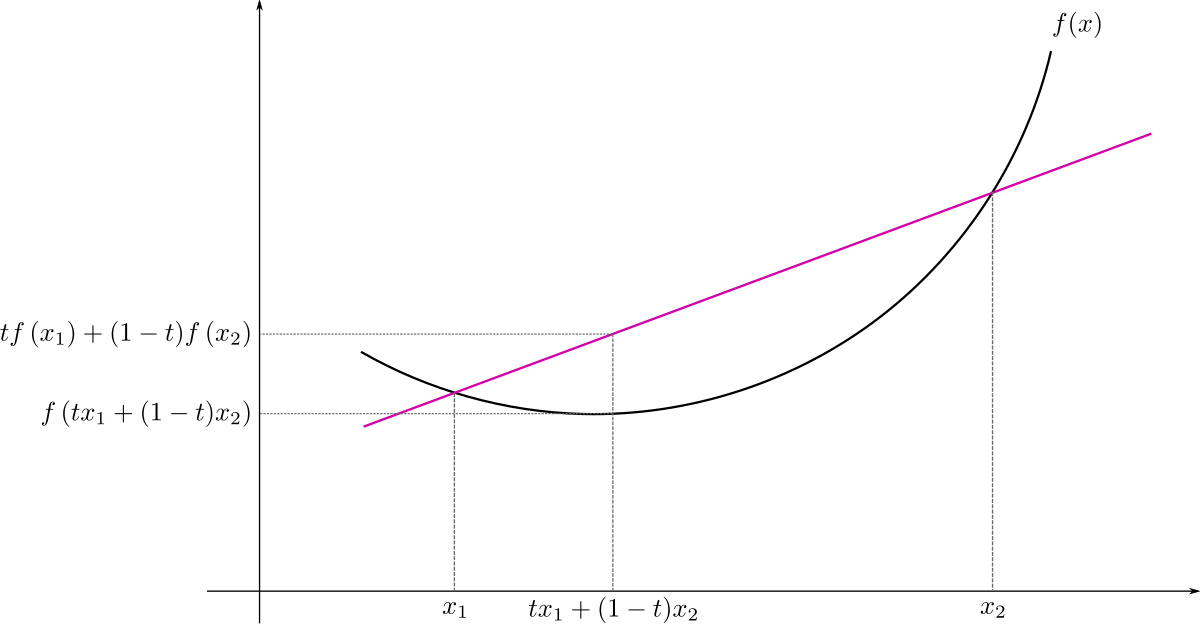
\includegraphics[width = 0.7\columnwidth]{figures/convexity.png}
	\end{center}
\subsection{Logistic Regression}

Choose $f(\boldsymbol{x})=\boldsymbol{w^Tx}+b$ and log-loss $l(t)=log(1+e^{-t})$:
\begin{emphbox}
$\min\limits_{\boldsymbol{w}\in\R^n,b\in\R}\frac{1}{n}\sum_{i=1}^nlog(1+exp(-y_i(\boldsymbol{w^Tx_i}+b)))$
\end{emphbox}
$P(Y=y|x)=\frac{1}{1+exp(-y(\boldsymbol{w^Tx}+b))}$, Prob. that y is correct\\
Find $\boldsymbol{w^*}, b^*$ by gradient descent\\
Classify new sample: $sign(\boldsymbol{w^{*T}x_{new}}+b^*)$

\subsection{Overfitting}
For linearly separable non empty training sets, the loss function has no global minimum in $\R^{p+1}$. If there is a dividing hyperplane (=lin. separable), we can scale its parameters and increase the value of the loss function. Dies does not need to be the best dividing hyperplane! Fixed by regularizer, e.g. adding $\lambda||\boldsymbol{w}||^2+b^2$

\subsection{Alternative Approach (Statistics)}
Linear Model: $a = w_0+w_1x_1+...+w_nx_m = \boldsymbol{w^Tx}$\\
\begin{tabular}{ll}
    Probability: $\sigma(a)=\frac{1}{1+e^{-a}}$ & $D=\{(\boldsymbol{x_i},z_i)\}$\\
    Find $\boldsymbol{w}_{MLE}=arg \max\limits_{\boldsymbol{w}} P(D|\boldsymbol{w})$ &  $\boldsymbol{x_i}\in \R^d, z_i\in\{0,1\}$\\
\end{tabular}
$P(D|\boldsymbol{w})=\prod\limits_{i=1}^n\sigma(\boldsymbol{w^Tx_i})^{z_i}(1-\sigma(\boldsymbol{w^Tx_i})^{1-z_i}$\\
$L(\boldsymbol{w}=-log(P(D|\boldsymbol{w})$, $\nabla_{\boldsymbol{w}}L(\boldsymbol{w})=\boldsymbol{X}(\sigma(\boldsymbol{X^Tw})-\boldsymbol{z})$\\
(Requires Hessian Matrix, which is positive semi-definite)\\
Results are identical up to the factor 1/n
\end{sectionbox}

\section{Kernels}
\begin{sectionbox}
Kernels replace the standard inner products with some function that is \emph{a suitable generalization of an inner product} to allow for nonlinear behavior.
\begin{emphbox}
    A positive semidefinite Kernel is a function $\kappa: \R^{p\times\p}\rightarrow\R$ so that for all sets $\mathbf{X}=\{\mathbf{x}_1,\cdot,\mathbf{x_n}\}$ the \emph{Gram-Matrix} $\mathbf{K}_{ij} = \kappa(\mathbf{x_i,x_j})$ is symmetric and positive semi definite  
\end{emphbox}
\begin{itemize}
    \item Symmetric: $\kappa(\mathbf{x_i,x_j})=\kappa(\mathbf{x_j,x_i}) \ \forall i,j$
    \item positive semi definite: $\mathbf{x^TKx}\ge 0\ \forall \mathbf{x}$ or all eigenvalues $\ge 0$
\end{itemize}
\subsection{Common Kernels and Rules}
\begin{itemize}
    \item Linear kernel: $\kappa(\mathbf{x,y}=\mathbf{x^Ty}+c, \ c\ge0$
    \item Polynomial Kernel $\kappa(\mathbf{x,y}=(a\mathbf{x^Ty}+c)^d,\ a,c,d\ge0 $
    \item Gaussian Kernel $\kappa(\mathbf{x,y}=exp(-\frac{||\mathbf{x-y}||^2}{2\sigma^2}$
    \item If $\kappa_1, \kappa_2$ are Kernels and $c\ge0$, then $c\kappa_1$, $c+\kappa_1$, $\kappa_1+\kappa_2$ and $\kappa_1\cdot\kappa_2$ are kernels as well
\end{itemize}
\end{sectionbox}

\section{Principal Component Analysis}
\begin{sectionbox}
\emph{Unsupervised Learning}: Structure unlabeled data. Here: reduce dimension of input without loosing to much information\\
Goal: Find $\boldsymbol{U}_k\in\R^{pxk}$ that minimizes $\sum\limits_{i=1}^n||\boldsymbol{x}_i-\boldsymbol{U_kU_k^Tx_i}||^2_2$
\subsection{PCA - Singular Value Decomposition}
Important: $\boldsymbol{X}$: centered observation matrix
SVD returns: $\boldsymbol{X} = \boldsymbol{XDV^T}$ with singular values $d_1\ge d_2\ge ... \ge d_n$ on the diagonal of \textbf{D}\\
$\boldsymbol{U_k}$ satisfies goal with diagonal covariance matrix $\boldsymbol{S}=\boldsymbol{U_k^TX}$\\
$s_{ij}$: j-th score of the i-th principal component. S: score matrix, U: loadings matrix\\
To reduced variables: $\boldsymbol{S} = \boldsymbol{D_kV_k^T}$, new sample: $s_{new}=\boldsymbol{U_k^T}s_{new}$\\
Cheaper than using $\boldsymbol{U_k^TX}$ ($nk$ operations instead $(2p-1)nk$\\
\emph{Dimensions}:\\ $X\in\R^{m\times n}$, $U\in\R^{m\times m}$, $D\in\R^{m\times n}$, $V^T\in\R^{n\times n}$, $U_k\in\R^{k\times n}$, $X_k\in\R^{k\times n}$, m: Dimension variable, n: samples\\
The eigenvectors of $\mathbf{X_aX_a^T}$ are the loadings of $\mathbf{X_a}$ only if $X_a$ is centered

\subsection{Statistical Interpretation}
Goal: Find $Y=\boldsymbol{U^T}X$ with $\boldsymbol{U^TU=I}$ and declining variance of the components

\subsection{Autoencoders}
Autoencoder: Form of neural networks, where input is first mapped to a lower dimension $k$ by $f$ and then back to input $g$: $g\circ f(x_i) \approx x_i$.
If $f$ and $g$ are linear and represented by $\boldsymbol{V}\in\R^{k\times p}$ and $\boldsymbol{W}\in\R^{p\times k}$ then $g\circ f(x_i)=\boldsymbol{WV}x_i$ and the error is measuered by the sum of squared distances $\sum_{i=1}^n||x_i-\boldsymbol{XV}x_i||^2$, then the first k singular vectors of \textbf{X} are optimal. \\
\textbf{WV} has at most rank k\\
If $f$, $g$ not linear: only approximation possible
\end{sectionbox}

\section{Kernel-PCA}
\begin{sectionbox}
\subsection{Linear PCA by inner products}
If $\mathbf{K}=\mathbf{X^TX}$ the inner product matrix and $\mathbf{X=U\SigmaV^T}$ the SVD of \textbf{X}, we can write $\mathbf{K=V\Sigma^T\Sigma V^T}$ with \textbf{$\Sigma^T\Sigma$} being diagonal. This is the eigenvalue decomposition of \textbf{X}\\
Let $\mathbf{V_k}$ and $\mathbf{\Sigma_k}=diag(\sigma_1, \cdots\sigma_k$ the first k eigenvectors and eigenvalues
\begin{emphbox}
    Therefore: $\mathbf{U_k^T}=\mathbf{\Sigma_k^{-1}V_k^TX^T}$ and for a new sample \textbf{y}:\\
    $\mathbf{U_k^Ty}=\mathbf{\Sigma_k^{-1}V_k^TX^Ty}=\mathbf{\Sigma_k^{-1}V_k^T}\mat{\mathbf{x_1^Ty} & \cdots \mathbf{x_n^Ty}}^T$\\
    This only requieres the inner product $\mathbf{x_n^Ty=k_y}$
\end{emphbox}
If \textbf{X} is not centered, we can center \textbf{K} without centering \textbf{X}:
\begin{center}
    $\mathbf{\tilde{K}=HKH}$ with $\mathbf{H}=(\mathbf{I}_n.\frac{1}{n}\mathds{1}_n\mathds{1}_n^T)$\\
    For new samples, we have to replace $\mathbf{\tilde{y}}=\mathbf{y}-\frac{1}{n}\mathbf{X}\mathds{1}_n$ and $\mathbf{\tilde{X}=XH}$\\
    $\mathbf{U_k^T}(\mathbf{\tilde{y}})=\mathbf{\Sigma_k^{-1}V_k^T\tilde{k}_y}$, \quad $\mathbf{\tilde{k}_y=Hk_y-}\frac{1}{n}\mathbf{HK}\mathds{1}_n$
\end{center}

\subsection{Transition to Kernel PCA}
Instead of replacing the inner product $\mathbf{x^Ty}$ by $\langle\phi(\mathbf{x}),\phi(\mathbf{y})\rangle$, we substitute $\mathbf{x^Ty}\rightarrow\kappa(\mathbf{x,y})$:
\begin{emphbox}
    $\mathbf{k}^{new}=\mat{kappa(\mathbf{x_1,y}) & \cdots & kappa(\mathbf{x_n,y})}^T$\\
    $\mathbf{k}_{cent}^{new}=\mathbf{Hk}_{cent}^{new}-\frac{1}{n}\mathbf{HK}\mathds{1}_n$
\end{emphbox}

\end{sectionbox}

\begin{sectionbox}

\begin{cookbox}{Kernel Principal Component Analysis}
        \item  for training set $\mathbf{X}=\mat{\mathbf{x}_1 & \cdots &\mathbf{x}_n}, \ \mathbf{x}_1\in\R^p$
		\item Find suitable Kernel function $\kappa(\cdot)$ and compute Gram Matrix $\mathbf{K}$
		\item Compute centered Gram Matrix: $\mathbf{\tilde{K}=HKH}$ with\\ $\mathbf{H=I}_n-\frac{1}{n}\mathds{1}_n\mathds{1}_n^T$
		\item Compute Eigenvalue Decomposition: $\mathbf{\tilde{K}=V\Lambda V^T}$. Because \textbf{K} is positive semi-definite and therefore the diagonal entries of $\mathbf{\Lambda}$ are non-negative, we write $\mathbf{\Lambda=\Sigma}^2=diag(\sigma_1^2, \cdot, \sigma_n^2)$
		\item Reduced Matrices: $\mathbf{\Sigma_k}=diag(\sigma_1,\cdots,\sigma_k),\ \in\R^{k\times k}$ and $\mathbf{V}_k\in\R^{n\times k}$
		\item Reduced Training Data: $\mathbf{S=\Sigma_kV}_k^T$
		\item For new datapoint $\mathbf{y}\in\R^p$, compute new components: 
		\begin{center}
		    $\mathbf{s}_new=\mathbf{\Sigma}_k^{-1}\mathbf{V}_k^T\mathbf{k}_{cent}^{new}$\\
		    $\mathbf{k}_{cent}^{new}=\mathbf{Hk}_{cent}^{new}-\frac{1}{n}\mathbf{HK}\mathds{1}_n$\\
		    $\mathbf{k}^{new}=\mat{kappa(\mathbf{x_1,y}) & \cdots & kappa(\mathbf{x_n,y})}^T$
		\end{center}
	\end{cookbox}
\end{sectionbox}

\section{Feedforward Neural networks}
\begin{sectionbox}
Minimize any expected loss at the price of training many parameters\\
Find $f\in \mathcal{F}$ that minimizes loss. If all functions in $\mathcal{F}$ can be described by a set of k parameters $\Theta\in\R^k$, then the goal is for N samples: \\
\begin{center}
    $\hat{\Theta}=arg\min\limits_{\Theta\in\R^k}=\frac{1}{N}\sum\limits_iL(f_\Theta(x_i))$
\end{center}
One layer of a FNN consists of a linear function $\varphi_{\boldsymbol{W}}(\boldsymbol{h})=\boldsymbol{Wh}$ and a nonlinear \emph{activation function}, e.g. the ReLU: $\sigma(t) = max\{0, t\}$:
\begin{center}
    $f:\R^p \rightarrow \R^k: \sigma_l\circ\varphi_{\boldsymbol{W_l}}\circ\cdots\circ\sigma_1\circ\varphi_{\boldsymbol{W_i}}(\boldsymbol{X})$
\end{center}
With $p$/$k$ Input/Output dimension and $l$ layers, \emph{Deep} FNN: $l>3$\\
$k$ depends on loss function (Output of FNN is input of Loss)

\subsection{Training FNNs (Backpropagation)}
\begin{emphbox}
        Functions $g:\R^k\rightarrow\R^l$ and $h:\R^l\rightarrow\R^m$ with $g$ being diff'able at \textbf{x} and $h$ at $\boldsymbol{y}=g(\boldsymbol{x})$ with Jacobi matrices $\boldsymbol{J}_g(\boldsymbol{x})$ and $\boldsymbol{J}_h(\boldsymbol{y})$ then\\
        $h\circ g:\R^k\rightarrow\R^m$ is diff'able at \textbf{x} with\\
        $\boldsymbol{J}_{h\circ g}(\boldsymbol{x})=\boldsymbol{J}_h(g(\boldsymbol{x})\cdot \boldsymbol{J}_g(\boldsymbol{x})$
\end{emphbox}
\end{sectionbox}

\section{Support Vector Machine (Basic Linear SVM)}
\begin{sectionbox}
    \begin{itemize}
        \item Idea: Find hyperplane to divide $\boldsymbol{x}, y$ into two subspaces
        \item Hyperplane: $\mathcal{H}_{\boldsymbol{w},b}=\{x\in \mathbb{R} | \boldsymbol{w^Tx}-b=0\}$, $\boldsymbol{w}$ normal to $\mathcal{H}$
        \item Euclidean distance from $\boldsymbol{x}$ to $\mathcal{H}_{\boldsymbol{w},b}$: $\delta(\boldsymbol{x}, \mathcal{H}_{\boldsymbol{w},b})=\frac{\boldsymbol{w^Tx}-b}{||\boldsymbol{w}||}$
        \item Goal: Find $y_i(\boldsymbol{w^Tx_i}-b)\ge 1\quad \forall i \in 1,...,N$
        \item Optimization Problem: $min \frac{1}{2}||\boldsymbol{w}||^2$ that fulfills Goal
    \end{itemize}
    \subsection{Karush Kuhn Tucker Conditions and Linear SVMs}
    \begin{emphbox}
    		$\min\limits_{\boldsymbol{w}, b, \boldsymbol{\lambda}\ge0} L(\boldsymbol{w}, b, \boldsymbol{\lambda})$ \\ 
    		$L(\boldsymbol{w}, b, \boldsymbol{\lambda})= \frac{1}{2}||\boldsymbol{w}||^2 - \sum\limits_i \lambda_i y_i(\boldsymbol{w^Tx_i}-b)+\lambda_i $\\
    		$\nabla_{(\boldsymbol{w},b)}L(\boldsymbol{w}, b, \boldsymbol{\lambda})=\mat{\boldsymbol{w}-\sum_i\lambda_iy_i\boldsymbol{x}_i \\ \sum_i \lambda_iy_i}$\\
			$\boldsymbol{w^*}=\sum_i\lambda^*_iy_i\boldsymbol{x}_i$  \quad $\sum_i \lambda^*_iy_i = 0$\\
			$L_D(\boldsymbol{\lambda})=\sum_i\lambda_i-\frac{1}{2}\boldsymbol{\lambda^TH\lambda}$ \quad With $h_{ij}=y_iy_x\boldsymbol{x_i^Tx_j}$\\
			New convex quadratic opt problem: $\boldsymbol{\lambda^*}=\max\limits_{\boldsymbol{\lambda}}L_D(\boldsymbol{\lambda})$
	\end{emphbox}
	\begin{itemize}
	    \item Problem is strictly convex, therefore solution is unique
	    \item If $\lambda_i \ne 0$, then $\boldsymbol{x_i}$ is support vector (Lies in or on margin)
	    \item Only works, if classes can be linearly separated 
	    \item Else: Kernel/Soft Margin SVM required
	    \item SVM works better when (nearly) separable than LR
	    \item SVM is preferred when using kernels compared to LR
	\end{itemize}
\end{sectionbox}

%  Lecture Notes Summary =======================================================================================================================

\newpage
\section{Decision Making}
\begin{sectionbox}
\begin{itemize}
\item \textbf{Decision making} is about mapping an input vector to an output value.
\item \textbf{Binary decision making} can be visualised via a joint pdf of X and Y, where Y takes on -1 or 1 and X  is a continuous random variable whose distribution changes conditioned on Y.
\item \textbf{Loss} is a positive, real measure of the deviation between a target and an output from a decision function.
\item \textbf{Expected prediction error} as a function of f is formulated by the expectation of the loss function, whose values change depending on the decision function f: $EPE(f)=E[L(Y, f(X))]$.
\item The aim of \textbf{global methods} is to find the best global decision function f out of class F that minimises the expected prediction error.
\item The aim of \textbf{local methods} is to find the best output which minimizes the expectation of loss on the distribution of Y conditioned on known X
\item We can obtain expected prediction error and expected loss due to the assumption that we \emph{know the joint pdf} of X and Y, i.e. the stochastic behaviour of the system.
\item For local methods with loss specified as the squared loss, expected loss is found to be the conditional expectation of of Y on the distribution of Y conditioned on X = x: $f(X)=E_{Y|X=x}[Y]$.
\item The problem with local methods is most of the time X is a continuous random variable and thus values here X=x are impossible, and so we take the \textbf{k-nearest neighbours} to x as approximations of x, thus giving us a set of samples representing the distribution of values X=x such that local method for finding output can now be applied to these samples.
\end{itemize}
\end{sectionbox}

\section{Curse of Dimensionality}
\begin{sectionbox}
\begin{itemize}
\item Most of the time it is desired that the dimensionality of samples are decreased due to various problems involved with working in high dimensions.
\item As the number of dimensions increases, the number of samples required to obtain an accurate representation of the probability distribution also increases a lot.
\item The \textbf{empty space theorem} says that as dimensionality increases, samples tend to be located at the tail end of their distributions.
\item As the number of dimensions increases, the distance between a point and any possible samples becomes more and more equidistant.
\item For a random vector $X\in\R^p$, the probability of at least one $X_i$ being further than $\beta$ away from the center: (For large $p$ this becomes 1)
\end{itemize}
\begin{emphbox}
$Pr(||X||^2_2\ge\beta)=1-Pr(X_1^2<\beta)^p$. 
\end{emphbox}
\end{sectionbox}

\section{Convex Functions}
\begin{sectionbox}
\begin{emphbox}
    \textbf{Definition Convexity}: $\mathcal{C}\subset\R^n$ a convex set, i.e for any pair $\boldsymbol{x_1,x_2}\in\mathcal{C}$ the point $t\boldsymbol{x_2}+(1-t)\boldsymbol{x_1} \in \mathcal{C} \ \forall t\in[0,1]$. A function is called \emph{convex} if $\forall \boldsymbol{x_1,x_2}\in \mathcal{C}, t\in[0,1]$:\\
    $tf(\boldsymbol{x_2})+(1-t)f(\boldsymbol{x_1}) \ge f(t\boldsymbol{x_2}+(1-t)\boldsymbol{x_1}) $
\end{emphbox}
\begin{itemize}
\item By definition, a function is convex if a line can be drawn between any two points in a function, and all vertical values of the line are greater than or equal to all vertical values of the function between the same two points.
\item A function is also convex if its second derivative is positive, or equivalently for vector inputs its Hessian matrix contains all non-negative eigenvalues.
\item Several operations between convex functions also result in another convex function, including the max between two convex functions:
\end{itemize}
\begin{emphbox}
    if $f,g$ convex, then: $max(f,g)$, $f+g$, $g\circ h$ (if g non-decreasing) are convex. Local minimum of \emph{strictly} convex is global minimum and unique
\end{emphbox}
\end{sectionbox}

\section{Logistic Regression}
\begin{sectionbox}
\subsection{Formulation via Optimization}
\begin{itemize}
\item The aim of logistic regression to perform binary classification on a random vector, that is, map a random vector to either -1 or 1.
\item In order to ensure that the outputs in logistic regression are either -1 or 1, the output in logistic regression is taken to be the sign of the output from a prediction function f which contributes to the decision.
\item The loss function in logistic regression is taken to be the number of misclassifications of a prediction, that is, 1 if the decision from logistic regression does not match the target, and 0 if it does match.
$f(z) = \left\{ \begin{array}{rcl}
     1 & \mbox{if}
& Y\cdot sign(f(x))\leq 0 \\ 0 & & \mbox{otherwise}\\
\end{array}\right.$
\item It is clear that we must find an appropriate f  to complete the decision function, and thus we define the global method with the \textbf{misclassification loss} as the problem we need to solve.
$ \frac{1}{n}\sum\limits_{i=1}^nL_{0,1}(y_i,f(x_i))$
\item The misclassification loss is extremely difficult to solve due to being non-continuous and non-convex, and so first we need to approximate this function as a convex function since they are easy to optimize.
\item A convex approximation of misclassification loss is $log(1 + exp(-t))$, which when concatenated with  an affine function $f(\boldsymbol{x})=\boldsymbol{w^Tx}+b$ is also convex, and can therefore be easily optimized via minimization.\\
\begin{center}
\begin{emphbox}
    $\min\limits_{\boldsymbol{w}\in\R^n,b\in\R}\frac{1}{n}\sum\limits_{i=1}^nlog(1+exp(-y_i(\boldsymbol{w^Tx}_i+b)))$
    \end{emphbox}
\end{center}
\item Noting that the loss is in \textbf{negative log-likelihood} form, we can convert this to a probability by taking the exponential of likelihood.
\begin{emphbox}
    \begin{center}
        $Pr(Y=y|x)=\frac{1}{1+exp(-y(\boldsymbol{w^Tx}+b}$
    \end{center}
\end{emphbox}
Gradient-based methods can be used to find affine weights and bias that optimize 3.3.
\end{itemize}
\subsection{Overfitting on Logistic Regression}
\begin{itemize}
\item When the samples are linearly separable, there is a constraint that the target times the affine output is always greater than zero Under this constraint, no global minimum exists.
\begin{emphbox}
    If the data is linearly separable, we can find ($\boldsymbol{w_s},b_s$) so that: $y_i(\boldsymbol{w_s^Tx_i}+b_s)<0 \ \forall i$\\
    then the lossfunction has no global minimum in $\R^{p+1}$
\end{emphbox}
\end{itemize}

\subsubsection{Proof}
This is proven by noting that for a global minimum to exist, a point with small, positive loss exists (3.17) such that all points have losses greater than or equal to this point (3.16). This has to be satisfied along the linearly seperable constraint (3.18). If this constraint is always satisfied, then (3.19) is always positive, which when subbed into (3.15) and scaling weights and bias to infinity we find that the loss approaches zero (3.21), thus violating the global minimum condition (3.18). This is prevented via regularization (3.23).
\end{sectionbox}

\begin{sectionbox}
\section{Principal Component Analysis}
PCA represents the data projected onto a lower-dimensional plane which captures most of the variance of the dataset.
\subsection{Geometric Interpretation}
\begin{itemize}
\item Imagining that $x$ is a vector in $p$ dimensions, and $U_k$ describes a lower dimensional subspace, then the coordinates of $x$ projected onto $U_k$ is found by first obtaining the scores of $x$ along $U_k$ and then taking the linear combination of these scores and the $U_k$ vectors: $\pi_\mathcal{U}(\boldsymbol{x})=\boldsymbol{U_kU_k^Tx}, \ \boldsymbol{U_k}\in\R^{p\times k}$
\item We want to find a $U_k$ that captures most of the variance in the dataset, which is equivalent to finding a hyperplane where the difference between the original data points and their projections are minimized, thus forming our problem for optimization.\\
\begin{center}
    $J(\boldsymbol{U_k})=\sum\limits_{i=1}^n||\boldsymbol{x_i}-\boldsymbol{U_kU_k^Tx_i}||^2_2$
\end{center}
\item The dataset can be represented as the dot product of an orthonormal matrix, a diagonal matrix and another orthonormal matrix via singular value decomposition: $\boldsymbol{X}=\boldsymbol{UDV}^T$.
\end{itemize}
\begin{emphbox}
    The first $k$ columns of the first orthonormal matrix via SVD $\boldsymbol{U_k}$ minimizes the the difference between data points and their projections, and the corresponding covariance matrix of the scores is diagonal (= features are uncorrelated).
\end{emphbox}
\begin{itemize}
\subsection{Proof}

\item Theorem 4.1 is proved by first reframing the minimization problem (4.2) into a maximization problem, reframing this again into a problem involving the trace of a rank k projection matrix, then noting that the maximum value along the diagonals is 1 (4.5) of which subbing in $U_k$ achieves due to its resulting in a identity matrix.
We can show that the scores are uncorrelated by showing that the dot product between the scores and its transpose scaled by 1/n is a diagonal matrix using the SVD. (4.6)
\item If we have the product between two matrices where the first matrix is is comprised of a diagonal matrix as well as a zero matrix, then we can get rid of the zero columns in the first matrix and also get rid of the corresponding rows in the left matrix.
\item A computationally inexpensive way of obtaining the scores using the singular values and right singular vector can be derived by substiuting the SVD into the formula for the calculating the scores. (4.7)
\end{itemize}

\subsection{Statistical Interpretation}
The idea behind the statistical interpretation is that covariance matrices are symmetric positive semidefinite, and therefore there exists some matrix U which can diagonalize it (clearly illustrated using the eigenvalue decomposition). Thus we can push U inside the covariance formula (4.8) to show that the scores with uncorrelated dimensions are obtained by projecting X onto U. (4.9)
\begin{emphbox}
        $\boldsymbol{D}=\boldsymbol{U^T}var(X)\boldsymbol{U} = E[\boldsymbol{U^T(x-\mu_x)(X-\mu_x)^T\boldsymbol{U}}]=E[(\boldsymbol{U^T}X-\boldsymbol{U^T}\mu_x)(\boldsymbol{U^T}X-\boldsymbol{U^T}\mu_x)^T]=E[(\boldsymbol{Y}-\mu_y)(\boldsymbol{Y}-\mu_y)^T=var(\boldsymbol{Y})$
\end{emphbox}
\subsection{Error Model Interpretation}
\begin{itemize}
\item The error model interpretation is that the samples $\boldsymbol{X}$ is obtained via the addition between a signal matrix $\boldsymbol{L}$ and a noise matrix $\boldsymbol{N}$, where $\boldsymbol{L}$ is lying on a lower dimensional subspace than $\boldsymbol{X}$, and the goal is to try and find $\boldsymbol{L}$.
Theorem 4.2
\item Setting $\boldsymbol{L}$ equal to the SVD ($p$ dimensions with $k$) minimizes the Frobenius norm of the difference between $\boldsymbol{X}$ and $\boldsymbol{L}$ given that the dimension $k$ of the subspace which $\boldsymbol{L}$ lies in is known beforehand.
\end{itemize}
\end{sectionbox}

\begin{sectionbox}
\subsection{Relation to Autoencoders}
\begin{itemize}
    \item Autoencoders map an input to low dimensional space using a function $f$, which is then mapped back to a higher dimensional space using a function $g$ and can approximate the input $g\circ f(\boldsymbol{x_i})\approx\boldsymbol{x_i}$
\item Letting $f$ and $g$ be linear mappings represented by matrices, the reconstruction error $J(\textbf{W,V})=\sum_{i=1}^n||\boldsymbol{x_i-WVx_i}||^2$ is minimised by setting $f$ as the transpose of $U_k$ and $g$ as $U_k$.
\begin{emphbox}
    Let \textbf{$U_k$} be the first $k$ left singular vectors of observation matrix \textbf{X}, the $\textbf{V}=\textbf{U}_k^T$ and $\textbf{W}=\textbf{U}_k$ minimize the reconstruction error of the linear autoencoder.
\end{emphbox}
\item This is proven by noting that in Theorem 4.2 which has a problem of the same form, the error is minimized using the projections of the points on the subspace of interest, thus leading to $f$ and $g$ as the transpose of $U_k$ and $U_k$ itself respectively as they cause this projection.

\end{itemize}
\end{sectionbox}

\section{Feed forward Neural Networks}
\begin{sectionbox}
\subsection{Definitions and Motivation}
The power behind an FNN is its ability to minimize any kind of expected prediction error, that is, find model parameters that minimize expected loss (5.1). Feed forward neural networks are concatenations of linear functions (5.2) with activation functions (e.g. 5.3), which can be denoted in vector form. This results in the generalized form of an FNN. (5.5)
\begin{emphbox}
    Given function class $\mathcal{F}$ described by set of k parameters $\Theta\in\R^<k$:\\
    Solve: $\hat{\Theta}=arg\min_{\Theta\in\R^k}=\frac{1}{N}\sum_iL(f_\Theta(\mathbf{x_i}))$ (5.1)\\
    $\varphi_\mathbf{W}:\R^p\rightarrow\R^m, \varphi_\mathbf{W}(\mathbf{h})=\mathbf{Wh}$ (5.2)\\
    $\sigma(t)=max\{0,t\}$ (ReLU, 5.3)\\
    $f:\R^p \rightarrow \R^k: \sigma_l\circ\varphi_{\boldsymbol{W_l}}\circ\cdots\circ\sigma_1\circ\varphi_{\boldsymbol{W_1}}(\boldsymbol{X})$(5.5)
\end{emphbox}
\subsection{Training FNN}
The gradients can be calculated via chain rule through each subsequent layer, or in this case due to vectors via the Jacobian. From (5.5) the key stages include matrix multiplication (5.2) and nonlinear activation (5.3). The corresponding Jacobians w.r.t. inputs in each stage is seen in (5.6) and (5.7) respectively. However, for the Jacobian of matrix multiplication w.r.t weights, the weights need to be reshaped into a vector (5.9) which will then allow us to formulate the Jacobian (5.10). Then the gradients w.r.t loss (5.11) is simply (5.31a). The gradient can then be used to update the weights for the next time step, making sure to apply an inverse reshaping of the gradient vector into a matrix (5.14).
\begin{emphbox}
    $\mathbf{J}_{\mathbf{W} g}(\mathbf{x})=\mathbf{W\cdot J_g}(\mathbf{x})$ (5.6)\\
    $\mathbf{j}_{(ij),\sigma}(\mathbf{x}) = \left\{ \begin{array}{rcl}
     \sigma'(x_i) & \mbox{if}
& i=j \\ 0 & & \mbox{else}\\
\end{array}\right.$ (5.7)\\
$\mathbf{J}_{mult}(x)=diag(\mathbf{x}^T)\in\R^{m\times mn}$ (5.10), doesn't depent on\\
With $\mathbf{h}_j=\sigma_j\circ\varphi_\mathbf{W_j}\circ\cdots\circ\sigma_1\circ\varphi_{\mathbf{W_1}}(\mathbf{x})$ the j-th output\\
We get for the output-layer (L): $\frac{\partial}{\partial\mathbf{W}_l}F=\mathbf{J}_L(\mathbf{h}_l)\cdot\mathbf{J}_{\sigma_l}(\mathbf{W_lh_{l-1}})\cdot\mathbf{J}_{mult}(\mathbf{h}_{l-1})$\\

$\frac{\partial}{\partial\mathbf{W}_j}F=\mathbf{J}_L(\mathbf{h}_l)\cdot\mathbf{J}_{\sigma_l}(\mathbf{W_lh_{l-1}})\cdot\mathbf{W_l}\mathbf{J}_{\sigma_{l-1}}(\mathbf{W_{l-1}h_{l-2}})\cdot\mathbf{J}_{l-1}\cdots \mathbf{J}_{mult}(\mathbf{h}_{l-1})$ for the j-th layer
\end{emphbox}
\end{sectionbox}

\section{Kernel Trick}
\begin{sectionbox}
\begin{itemize}
\item A kernel is a function that maps two sets containing real numbers (representing a sample) to a single scalar, such that for all possible sets of samples (contained in a data matrix with columns corresponding to samples) the Gram-Matrix (6.1) is symmetric and positive semidefinite.
\begin{emphbox}
    A positive semidefinite Kernel is a function $\kappa: \R^{p\times\p}\rightarrow\R$ so that for all sets $\mathbf{X}=\{\mathbf{x}_1,\cdot,\mathbf{x_n}\}$ the \emph{Gram-Matrix} $\mathbf{K}_{ij} = \kappa(\mathbf{x_i,x_j})$ is symmetric and positive semi definite  
\end{emphbox}
\item We can determine whether a particular function is a kernel by testing for violations of symmetry or positive semidefiniteness.
Symmetry can easily be tested by substituting named variables into the kernel, then flipping around the variables and seeing whether the kernel expression is the same.
\item Positive semidefiniteness can be tested as violated by definition, or if any diagonal values are ever negative. Furthermore, if the determinant of a matrix is negative it is definitely not psd (since psd eigenvalues are nonnegative and the determinant is the product of the eigenvalues), but we cannot say anything if the determinant is positive.
\end{itemize}
\end{sectionbox}

\section{Kernel PCA}
\begin{sectionbox}
\subsection{Linear PCA with Inner Products}
\begin{itemize}
\item Scores of the input data can be calculated using singular values and the right eigenvector (4.7), which we can obtain using the eigenvalue decomposition of the Gram-Matrix (7.2) and therefore giving us a way to calculate linear PCA scores using the inner product. If we forgot to center the data, use the centred Gram-Matrix instead (7.8).

\item If the input data has not been centred beforehand, we can find the Gram-Matrix for the centred data by noting how input data is usually centred (7.6), factoring out the input matrix (7.7) and then using inner product to compute the Gram-Matrix  corresponding to centred input. (7.8)
\item Scores for new observations are usually calculated by projecting them onto $U_k$, but if we want to reformulate this to be in terms of the singular value and right singular vectors we can isolate U in the SVD and retain only k columns (7.4a) to arrive at the formulation. (7.4)
\item If we want to calculate scores for new observations considering centering, we take the formula for raw new observations (7.4), replace the input matrix with a centred input matrix and the observation with an approximated centred observation, resulting in a nice formula involving the Gram-Matrix. (7.9)
\begin{emphbox}
    EVD of Gram Matrix (7.2): $\mathbf{K=V\Sigma^T\Sigma V^T}$\\
    Centered Gram Matrix (7.8): $\mathbf{\tilde{K}=HKH}$ with $\mathbf{H}=(\mathbf{I}_n.\frac{1}{n}\mathds{1}_n\mathds{1}_n^T)$\\
    Computing scores for new sample $\mathbf{y}$:
    $\mathbf{U_k^T}(\mathbf{\tilde{y}})=\mathbf{\Sigma_k^{-1}V_k^T\tilde{k}_y}$, \quad $\mathbf{\tilde{k}_y=Hk_y-}\frac{1}{n}\mathbf{HK}\mathds{1}_n$
\end{emphbox}
\subsection{Transition to Kernel PCA}
\item Kernel PCA requires us to first compute the Gram-Matrix via the kernel (6.1). This can then be substituted for the Gram-Matrix via inner product at various places, such as during centering (7.8) and when performing eigenvalue decomposition (7.2) to calculate matrices for scores (4.7).
\item The scores for new observations via Kernel PCA is based off the Linear PCA version (7.4), and can be obtained by replacing the linear observation inner products with the kernel observation inner products (as well as ensuring that singular values and right singular vectors obtained from eigenvector decomposition of Gram-Matrix via kernel (7.2)).
\item Similarly, when considering centering, note the Linear PCA version of scores which consider centering (7.9) and replace the linear Gram-Matrix with the kernel Gram-Matrix as well as the linear observation inner products with the kernel observation inner products. (7.12)
\end{itemize}
\end{sectionbox}

\section{Support Vector Machines}
\begin{sectionbox}
\begin{itemize}
\subsection{Geometry}
\item For some vector w, an affine hyperplane is described as the set of points x that can be projected onto w and then shifted by some constant b to equal zero. (8.1)
\item The vector w is normal to the hyperplane (8.1) since a vector of any direction in the hyperplane projected onto w has a magnitude of zero. (8.2)
\item The signed distance from any point to a hyperplane is defined as in (8.3), and can be interpreted as the distance from the hyperplane to the point x. It is formulated by first projecting x onto w and then centering the number line at b to obtain the signed value of x in the decision perspective (denote this as the decision distance). Then this value is divided by the magnitude of w to obtain the signed distance. Note that -b denotes the decision distance to the origin, and the magnitude of w is a scaling factor used to shift between the decision distance and signed distance.
\begin{emphbox}
    Hyperplane:$\mathcal{H}_{\boldsymbol{w},b}=\{x\in \mathbb{R} | \boldsymbol{w^Tx}-b=0\}$ (8.1)\\
    \textbf{w} is normal to $\mathcal{H}$: $\mathbf{w}^T(\mathbf{x_1-x_2})=0$ (8.2)\\
    Signed Distance: $\delta(\boldsymbol{x}, \mathcal{H}_{\boldsymbol{w},b})=\frac{\boldsymbol{w^Tx}-b}{||\boldsymbol{w}||}$ (8.3)\\
    Margin:$\mathcal{H}_{+}=\{x\in \mathbb{R} | \boldsymbol{w^Tx}-b=1\}$ $\mathcal{H}_{-}=\{x\in \mathbb{R} | \boldsymbol{w^Tx}-b=-1\}$ (8.8-9)
    
\end{emphbox}
\item The decision perspective can be imagined as the perspective where classification decisions are made, all depending on the decision distance.
\item The positive margin is defined as the hyperplane with a decision distance of 1 (8.8), and the negative margin is defined as the hyperplane with a decision distance of -1 (8.9).
\subsection{Basic Linear SVM}
\item The aim of Linear SVM is to linearly separate data using the margins of the hyperplanes, such that all positively labelled data is bounded by the positive margin and all negatively labelled data is bounded by the negative margin. In other words, all positively labelled data has a decision distance greater than or equal to 1, and all negatively labelled data has a decision distance less than or equal to -1, resulting in a separation constraint for w and b. (8.12)
\item We define the best w and b as the ones that have the widest margin, i.e. the widest distance between the hyperplanes. This width his calculated by the sum of the signed distance from the positive margin to the hyperplane and the signed distance from the hyperplane to the negative margin (8.13), which we can then maximize subject to our separation constraint (8.12). \item Flipping around the numerator and denominator of the width, this becomes a minimization problem (8.14).
\begin{emphbox}
    Conditions: $\mathbf{w^Tx}_i-b\ge +1 \ \mbox{for } y_i=
    1$ and $\mathbf{w^Tx}_i-b\ge -1 \ \mbox{for } y_i=
    -1$\\
    Compact: $y_i\cdot(\mathbf{w^Tx}_i-b)\ge1 \ \forall i$ (8.12)
    Minimization: $\min\limits_\mathbf{w}\frac{1}{2}||\mathbf{w}||^2_2 \ \mbox{s.t.} \ y_i(\mathbf{w^Tx}_i-b)\ge1 \ \forall i$
\end{emphbox}
\end{itemize}
\end{sectionbox}

\begin{sectionbox}
\begin{itemize}
\subsection{KKT and Lagrangian Duality}
\item The Karush-Kuhn Tucker conditions says that a minimisation problem with a set of equality and inequality constraints (8.15) can be reformulated as a Lagrangian primal (8.16) with some KKT conditions (Theorem 8.2), such that for convex objective functions with a convex feasible region (like that defined 8.14) minimising the primal (8.16) is equivalent to minimising the original problem (8.15).
\begin{emphbox}
    For a optimization problem with $\mathcal{E}$ and $\mathcal{I}$ as \emph{equality and inequality constraints} (8.15):\\
    $\min\limits_{\mathbf{z}\in\R^n}f(\mathbf{z}) \ \mbox{s.t. } c_i(\mathbf{z}) = 0 \ \forall i\in\mathcal{E} \ \mbox{and s.t. } c_j(\mathbf{z}) \ge 0 \ \forall j\in\mathcal{I}$\\
    Lagrange Function (8.16): $L(\mathbf{z,\lambda})=f(\mathbf{z})-\sum\limits_{i\in\mathcal{I}\bigcup\mathcal{E}}\lambda_ic_i(\mathbf{z})$
    \textbf{Karush-Kuhn-Tucker Conditions}\\
    For $\mathbf{z^*}$ as a solution to 8.15, there exists a larange multiplier $\mathbf{\lambda^*}$ such that:\\
    \begin{itemize}
        \item $\Delta_zL(z^*,\lambda^*)=0$
        \item $c_i(z^*)=0 \quad \forall i\in\mathcal{E}$
        \item $c_i(z^*)\ge0 \quad \forall i \in\mathcal{I}$
        \item $\lambda_i^* \ge0 \quad \forall i\in\mathcal{I}$
        \item $\lambda_i^*c_i(z^*)=0 \quad \forall i\in\mathcal{I}\bigcup\mathcal{E}$
    \end{itemize}
\end{emphbox}
\item The convex primal function (8.16) can then be reformulated as a concave dual function (8.22) by taking the infimum of the primal function. The infimum is the set of points along which the function is minimized w.r.t. the non-Lagrangian multiplier variables. Then by maximizing the primal subject to its constraints (8.22a) we obtain a lower bound for the solution to the primal (weak duality) or when some conditions are satisfied (such as in SVM) this coincides with the solution to the primal (strong duality).
\subsection{Linear SVM via Lagrangian Duality}
\item SVM via Lagrangian duality follows the process specified above. The original problem is as in (8.14), the Lagrangian primal is as in (8.23 to 8.25) and the KKT conditions are as in (8.26 to 8.29). 
\begin{emphbox}
    Problem: $\min\limits_{\boldsymbol{w}, b, \boldsymbol{\lambda}\ge0} L(\boldsymbol{w}, b, \boldsymbol{\lambda})$ \\  $L(\boldsymbol{w}, b, \boldsymbol{\lambda})= \frac{1}{2}||\boldsymbol{w}||^2 - \sum\limits_i \lambda_i y_i(\boldsymbol{w^Tx_i}-b)+\lambda_i $\\
    		$\nabla_{(\boldsymbol{w},b)}L(\boldsymbol{w}, b, \boldsymbol{\lambda})=\mat{\boldsymbol{w}-\sum_i\lambda_iy_i\boldsymbol{x}_i \\ \sum_i \lambda_iy_i}$\\
    KKT Conditions:\\ $\mathbf{w^*}-\sum_i\lambda_i^*y_ix_i=0$, \quad $\sum_i\lambda^*_iy_i=0$\\
    $\lambda_i^*(y_i(w^{*T}x_i-b^*)-1=0$\\
    Returns: \\
    $\min\limits_{\boldsymbol{w}, b, \boldsymbol{\lambda}\ge0} L(\boldsymbol{w}, b, \boldsymbol{\lambda})=L_D(\mathbf{\lambda})=
    \sum\limits_i\lambda_i-\frac{1}{2}\sum\limits_{i,j}\lamda_i\lambda_jy_iy_j\mathbf{x_i^Tx_j}$ s.t. $\lambda_i\ge0, \ \sum_i\lambda_iy_i=0$
\end{emphbox}

\item Then the dual function needs to be calculated by taking the infimum of 8.25, which is accomplished by substituting the gradients w.r.t w and b (8.26) inside, resulting in the dual function (8.30a).
\item Maximising this function w.r.t. its constraints is then the dual problem for SVM. (8.30)
\end{itemize}

\end{sectionbox}

\section{Useful Facts}
The matrix resulting from the dot product of between an $R^{n x p}$ matrix and $R^{p x n}$ has at most a rank of p.


\newpage
\section{Homework and Assignments}
Given a prediction table, eg:
\begin{tabular}{l|c|r}
    $p_X(X_1,X_2)$& $X_2=0$ & $X_2=1$ \\
    \hline
     $X_1=0$& $p_X(0,0)$& $p_X(0,1)$ \\
     \hline
     $X_2=1$& $p_X(1,0)$& $p_X(1,1)$
\end{tabular}
    \begin{cookbox}{Calculate Covariance Matrix from Table}
            \item Calculate Means for $X_1$ and $X_2$: $\mu_1, \mu_2$
            \item Create X-Matrix, e.g.: \mat{0 & 1 & 0 & 1\\ 0 & 0 & 1 & 1}
            \item Create p-Matrix: \mat{$p_X(0,0)$ & 0 & 0 & 0 \\
                                        0 & $p_X(1,0)$ & 0 & 0 \\
                                        0 & 0 & $p_X(0,1)$ & 0 \\
                                        0 & 0 & 0 & $p_X(1,1)$}
            \item Calculate Covariance: $Cov=XpX^T$
    \end{cookbox}
\begin{sectionbox}
\subsection{Classification Analysis}

\subsubsection{ROC Curve}
The ROC curve is a graphical plot that illustrates the diagnostic ability of a binary classifier system as its discrimination threshold is varied. It shows:
\begin{itemize}
    \item The relationship between sensitivity and specificity. For example, a decrease in sensitivity results in an increase in specificity.
    \item Test accuracy; the closer the graph is to the top and left-hand borders, the more accurate the test. Likewise, the closer the graph to the diagonal, the less accurate the test. A perfect test would go straight from zero up the the top-left corner and then straight across the horizontal.
    \item The likelihood ratio; given by the derivative at any particular cutpoint.
\end{itemize}
\begin{center}
	    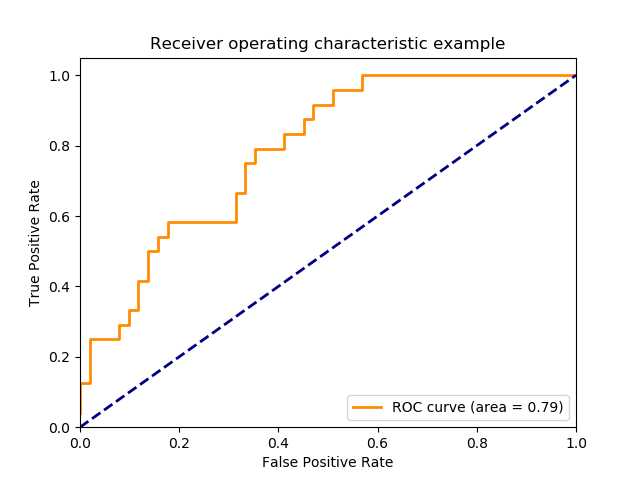
\includegraphics[width = 0.9\columnwidth]{figures/sphx_glr_plot_roc_001.png}
	\end{center}
The \textbf{Area under the Curve (AUC)} is the integral of the ROC Curve and gives a measure how good the classifier is. An area under the ROC curve of 0.8, for example, means that a randomly selected case from the group with the target equals 1 has a score larger than that for a randomly chosen case from the group with the target equals 0 in 80\% of the time. When a classifier cannot distinguish between the two groups, the area will be equal to 0.5 (the ROC curve will coincide with the diagonal). When there is a perfect separation of the two groups, i.e., no overlapping of the distributions, the area under the ROC curve reaches to 1 (the ROC curve will reach the upper left corner of the plot). 
\end{sectionbox}

\begin{sectionbox}
\subsection{Curse of Dimensionality}
\begin{itemize}
    \item The angular distance between $2$ randomly sampled vectors increases with dimension $d$ of the sample space.
\item Convergence to $\frac{\pi}{2}$ implies that two randomly sampled vectors are orthogonal to each other in $d$-dimensional apsce for $d\gg n$.
\item Convergence to $\frac{\pi}{2}$ also implies that most samples are concentrated in the 'corners' of the $d$-dimensional cube $[-1, 1]^d$, i.e. in high dimension, the corners occupy most of the space.
\item This convergence also means that $2$ randomly sampled vectors are increasingly equidistant (in termas of angular distance) from their respective nearest neighbors in high dimensional space.
\item Because the samples are increasingly equidistant from each other, this means that distance-based classifiers (e.g. k-Nearest Neighbors) cannot be used on such data in high-dimensional space.
\item Increasing the sample size $n$ decreases the average angular distance between neighbouring vectors in a $d$-dimensional feature space. The rate of decrease, however, decreases with increasing $n$.
\end{itemize}

\begin{center}
	    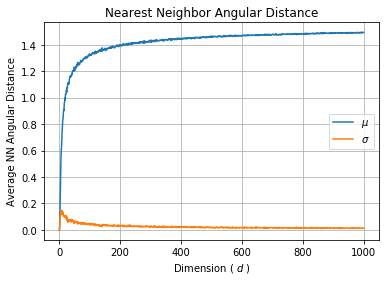
\includegraphics[width = 0.9\columnwidth]{figures/angular_distance_plot.png}
	\end{center}
\end{sectionbox}

\begin{sectionbox}
 \subsection{Logistic Regression}
 \begin{itemize}
     \item  With big datasets, standard gradient descent could lead to       \texttt{Memory Error}
     \item Use \emph{stochastic gradient descent} instead: Train over epochs instead:
     \item Each epoch, the training set is divided randomly into equal size subsets (=minibatch). Then the gradient of each subset is calculated and applied only to the samples in the subset
     \item A epoch is finished when the gradient step was performed on each subset

 \end{itemize}
\end{sectionbox}

\begin{sectionbox}
\subsection{Principal Component Analysis}
Removing the first $n$ columns from $U_k$ can have different effects on classification:
\begin{itemize}
    \item \textbf{Decreased Error Rate}: This may be because even though the first $n$ components capture more variance in the samples, perhaps the other components are better at separating samples by labels, allowing KNN to correctly classify samples (Subset 1 in top plot and second plot)
    \item \textbf{No Effect on Error Rate}: This may be because the first three principal components are as good at separating samples by labels compared to other principal components (Subsets 2+3 in top plot and third plot)
    \item \textbf{Increase Error Rate}: This may be because the first three principal components are better at separating samples by labels compared to the other principal components (Subset 4 top plot and bottom plot)
\end{itemize}
\subsubsection{How to choose $k$?}
Assuming that $\mathbf{X} \in \mathbb{R}^{p \times N}$ is the centered data matrix and $\mathbf{P} = \mathbf{U}_k \mathbf{U}_k^\top$ is the projector onto the $k$-dimensional principal subspace, the dimension $k$ is chosen such that the fraction of overall energy contained in the projection error does not exceed $\epsilon$, i.e.\
	\begin{equation*}
	    \frac{\|\mathbf{X} - \mathbf{PX}\|_F^2}{\|\mathbf{X}\|_F^2} 
	    = \frac{\sum_{i=1}^{M} \|\mathbf{x}_i - \mathbf{Px}_i\|^2}{\sum_{i=1}^N \|\mathbf{x}_i\|^2} \leq \epsilon,
	\end{equation*}
where $\epsilon$ is usually chosen to be between 0.01 and 0.2. Energy is not always the best way to measure useful information, e.g. when images differ in brightness (=No use full information)
\end{sectionbox}

\begin{center}
	    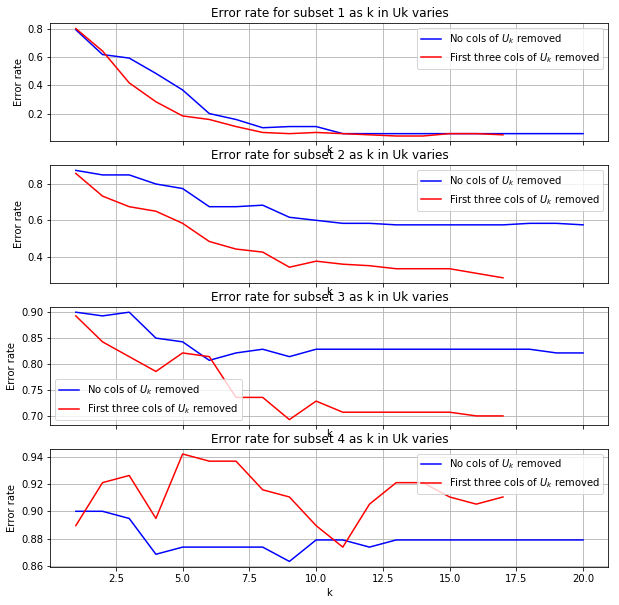
\includegraphics[width = 0.9\columnwidth]{figures/error_if_removed.png}
	\end{center}
\begin{center}
	    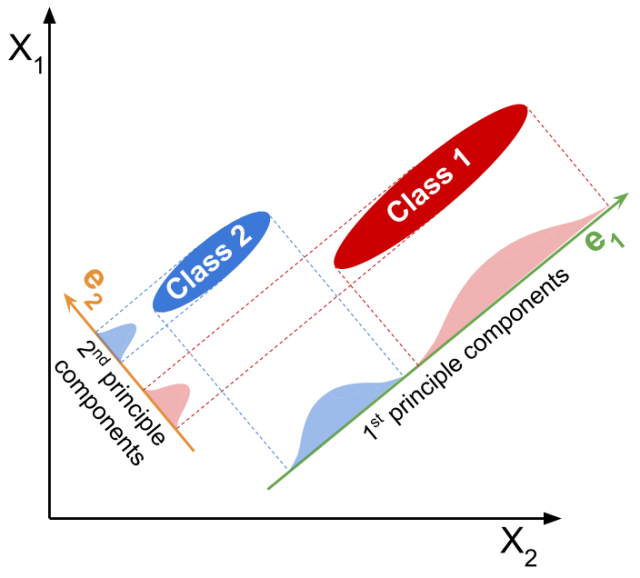
\includegraphics[width = 0.7\columnwidth]{figures/PCA_case1.png}
	\end{center}
\begin{center}
	    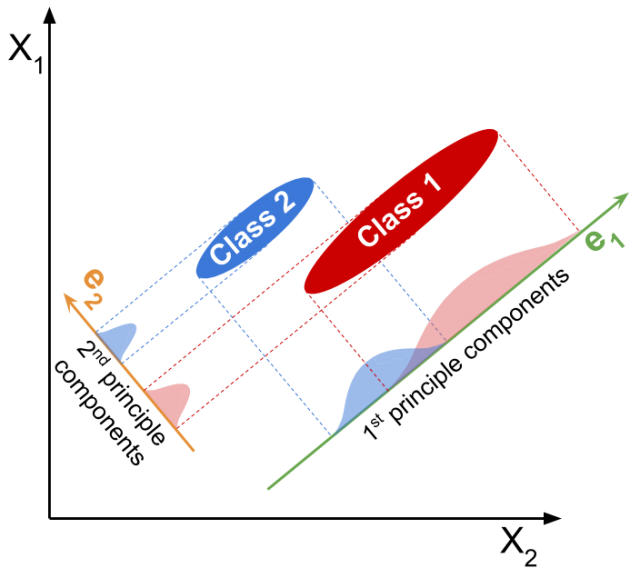
\includegraphics[width = 0.7\columnwidth]{figures/PCA_case2.png}
	\end{center}
\begin{center}
	    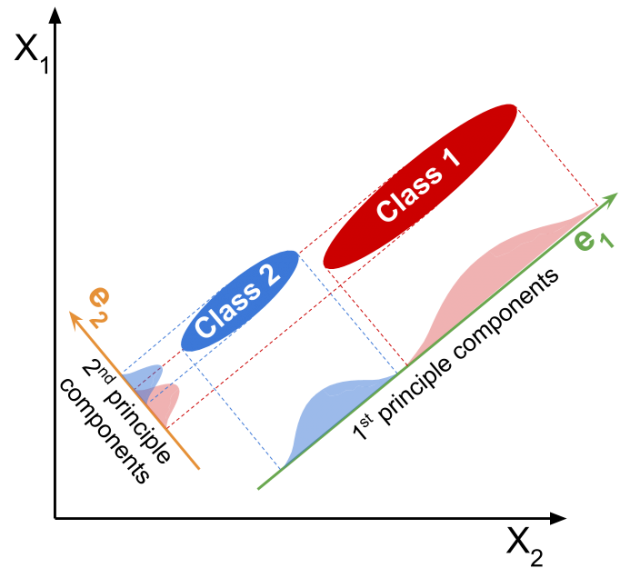
\includegraphics[width = 0.7\columnwidth]{figures/PCA_case3.png}#
	\end{center}
% DOCUMENT_END =================================================================
\end{document}
